\chapter{Perceiving: Supplemental Information}
\label{app:perception}

\section{Method for Methane Measurement from Niskin Bottles}
\label{app:perception:methane}
A Los Gatos Research (LGR) Dissolved Gas Extraction Unit (DGEU) and Greenhouse Gas Analyzer (GGA) were used to process water collected by Niskin bottle samples during the transect, and report methane concentration estimates to be compared to the \emph{in situ} observation of normalized methane by SAGE mounted on the rosette. Measurements of methane made by the GGA are reported as the stabilized parts per million (ppm) reading provided by the instrument after consuming 3-5 L of seawater from each Niskin bottle, and are converted to nanomolar (nM) values by first computing the partial pressure of methane, and then computing molarity by estimating the solubility constant of methane using coincident measurements of salinity and temperature of the seawater at time of bottle sample collection as measured by the rosette CTD. The conversion from partial pressure to molarity is done using the \verb|gasex| Python library, publicly hosted at \url{https://github.com/boom-lab/gasex-python}. 

To transform GGA measurements in ppm to partial pressure, the DGEU cell pressure is used, such that $\text{ppm} \times \text{cell pressure} = \text{partial pressure}$. Additionally, gas extraction inefficiency is taken into consideration at this step; the DGEU does not perfectly extract gas across the membrane during sampling. Extraction efficiency is used to scale the GGA measurement of methane prior to computing the partial pressure estimate by 

\begin{equation}
    \label{eq:extraction}
    \left[\frac{x_{obs} - x_{ref}}{\lambda_{eff}} + x_{ref}\right]\frac{p_{cell}}{1000} = x_{pp}
\end{equation}

\noindent where $x_{obs}$ is the ppm measurement made by the GGA, $x_{ref}$ is a methane reference value (the atmospheric concentration of methane, typically between 1.86-1.99 ppm), $\lambda_{eff}$ is the extraction efficiency, $p_{cell}$ is the cell pressure in millibar, and $x_{pp}$ is the estimated partial pressure value, in $\mu$atm. 

The extraction efficiency used in this manuscript was estimated by laboratory calibrations to be between 2.3-3.3\%, consistent across different water temperatures and different test tank concentrations. In the laboratory calibration procedure, methane was bubbled in a temperature-controlled tank which was stirred before two discrete samples were taken using 60 mL syringes filled with 40 mL of water, and 20 mL of pure nitrogen gas. A DGEU, connected to the GGA, was then used to take water from the target tank, and ppm measurements by the GGA were recorded when measurements stabilized; this was done with two different DGEUs, which we label A and B. To estimate ``ground truth'' partial pressure of methane in the tank, the syringe samples were shaken for 2 minutes to extract the dissolved gas content, and the water drained. The samples were then processed within 24 hours on a gas chromatography instrument (Shimadzu GC-14B), run alongside a set of standards processed every 5 minutes. The measurements from the processed syringes (DGEU influent) were used as $x_{pp}$ in Eq.~\ref{eq:extraction}, the GGA observations as $x_{obs}$, the value 1.99 ppm used as $x_{ref}$, and 495 mbar as $p_{cell}$. The relevant data from these calibrations is available in Tab.~\ref{tab:extraction}. DGEU A was the instrument used in the transect field mission as presented in this manuscript.

\begin{table}[h!]
    \centering
    \begin{tabular}{c|c|c|c|c}
        DGEU & Temperature (C) & Influent ($\mu$atm) & GGA Methane (ppm) & Efficiency  \\
        \hline
        \hline
        & & & & \\
        A & 4.7 & 299.13 & 21.82 & 3.29\% \\
        A & 4.7 & 512.03 & 6.44 & 0.4\% \\
        A & 4.7 & 588.25 & 41.04 & 3.29\% \\
        B & 4.7 & 299.13 & 17.77 & 2.62\% \\
        B & 4.7 & 512.03 & 25.68 & 2.29\% \\
        B & 4.7 & 588.25 & 30.09 & 2.37\% \\
        A & 9.9 & 267.14 & 17.02 & 2.80\% \\
        A & 9.9 & 403.45 & 27.84 & 3.18\%  \\
        A & 9.9 & 856.89 & 55.77 & 3.11\% \\
        B & 9.9 & 267.14 & 12.72 & 2.00\% \\
        B & 9.9 & 403.45 & 18.63 & 2.05\% \\
        B & 9.9 & 856.89 & 36.99 & 2.02\% \\
        A & 14.8 & 18.64 & 2.78 & 2.22\% \\
        A & 14.8 & 1549.18 & 101.26 & 3.17\%  \\
        A & 14.8 & 1640.81 & 100.41 & 2.97\% \\
        B & 14.8 & 18.64 & 2.63 & 1.80\% \\
        B & 14.8 & 1549.18 & 78.93 & 2.46\% \\
        B & 14.8 & 1640.81 & 68.43 & 2.01\% \\
        & & & & \\
        
    \end{tabular}
    \caption{Results of DGEU extraction efficiency calibration experiments.}
    \label{tab:extraction}
\end{table}



\section{Leg 2 Niskin Bottle Sample Schedule and Measurements}
\label{app:perception:niskin}
This manuscript presents methane and ammonium measurements collected by Niskin bottles during Leg 2 of the rosette trajectory. Table~\ref{tab:niskin_sched} provides the schedule of Niskin bottle firing performed during Leg 2, and Table~\ref{tab:niskin_sched_results} provides all data associated with those bottles collected and presented in Chapter 3 of this thesis. The range of methane nM values is provided by converting GGA methane ppm measurements as described in Sec.~\ref{app:perception:methane} for the conservative range of valid DGEU extraction efficiency values.
\begin{table}[h!]
    \centering
    \begin{tabular}{c|c|c|c}
        Bottle & Time & Location & Depth (m) \\
        \hline
        \hline
        &&&\\
        1 & 2021-11-30 09:10:03 & 27.3951N 111.3649W & 1648.62 \\
        3 & 2021-11-30 09:30:03 & 27.3956N 111.3665W & 1625.67 \\
        5 & 2021-11-30 09:47:01 & 27.3967N 111.3696W & 1639.25 \\
        7 & 2021-11-30 09:47:05 & 27.3967N 111.3696W & 1639.05 \\
        9 & 2021-11-30 10:07:00 & 27.3985N 111.3740W & 1598.32 \\
        11 & 2021-11-30 10:17:02 & 27.2994N 111.3765W & 1580.5 \\
        13 & 2021-11-30 10:27:01 & 27.4005N 111.3791W & 1568.27 \\
        15 & 2021-11-30 10:27:04 & 27.4005N 111.3791W & 1568 \\
        17 & 2021-11-30 10:37:20 & 27.4016N 111.2818W & 1558.64 \\
        19 & 2021-11-30 10:46:59 & 27.4027N 111.3845W & 1553.92 \\
        21 & 2021-11-30 11:07:05 & 27.4051N 111.3900W & 1547 \\
        23 & 2021-11-30 11:33:00 & 27.4082N 111.3971W & 1545.4 \\
        &&&
    \end{tabular}
    \caption{Schedule of bottle samples during Leg 2 of rosette trajectory.}
    \label{tab:niskin_sched}
\end{table}

\begin{table}[h!]
    \centering
    \begin{tabular}{c|c|c|c|c|c}
        Bottle & CH$_4$ (ppm) & CH$_4$ (nM) & NH$_4^+$ (nM) & Temp. (C) & Salinity (PSU) \\
        \hline
        \hline
        &&&&&\\
        1 & -- & -- & 0.00 & 2.8334 & 34.6104 \\
        3 & 9.29 & 207-296 & 46.35 & 2.8578 & 35.6095 \\ 
        5 & 21.6 & 547-785 & -- & 2.8458 & 34.6107 \\
        7 & -- & -- & 174.48 & 2.8461 & 34.6108 \\
        9 & 22.54 & 573-821 & 165.99 & 2.8659 & 34.6101 \\
        11 & 29.82 & 774-1110 & 225.87 & 2.8719 & 34.6096 \\
        13 & 44.36 & 1176-1686 & -- & 2.8734 & 34.6099 \\
        15 & -- & -- & 384.28 & 2.8733 & 34.6098 \\
        17 & 89.45 & 2421-3473 & 780.53 & 2.8849 & 34.6105 \\
        19 & 114.27 & 3105-4454 & 997.45 & 2.8968 & 34.6111 \\
        21 & 27.29 & 704-1009 & 227.54 & 2.8835 & 34.6087 \\
        23 & 11.5 & 268-384 & 89.29 & 2.8964 & 34.6075 \\
        &&&&&
    \end{tabular}
    \caption{Geochemical measurements associated with the schedule of bottle samples during Leg 2 of rosette trajectory. Note that methane expressed in nM is computed using coincident temperature and salinity measurements during the transect as measured by rosette CTD, and extraction inefficiency of the DGEU is compensated for as described in Sec.~\ref{app:perception:methane}.}
    \label{tab:niskin_sched_results}
\end{table}


\section{Normalized Pythia Calibration}
\label{app:perception:norm}
The Pythia instrument provides a significantly nonlinear output reference value when measuring methane. We correct for this nonlinearity using a reference curve computed in the laboratory before normalizing the measurements as reported in this manuscript. The reference curve was created using a temperature-fixed (\SI{3}{\celsius}) tank and closed equilibriation chamber, in which methane standards were bubbled until fully equilibriated before being measured by the instrument. Stable measurements by Pythia (which has a response time of approximately 35 minutes) were then recorded at different chamber concentrations. The calibration curve that results is a piece-wise linear function, shown in Fig.~\ref{fig:nopp_curve}.

\begin{figure}[h!]
    \centering
    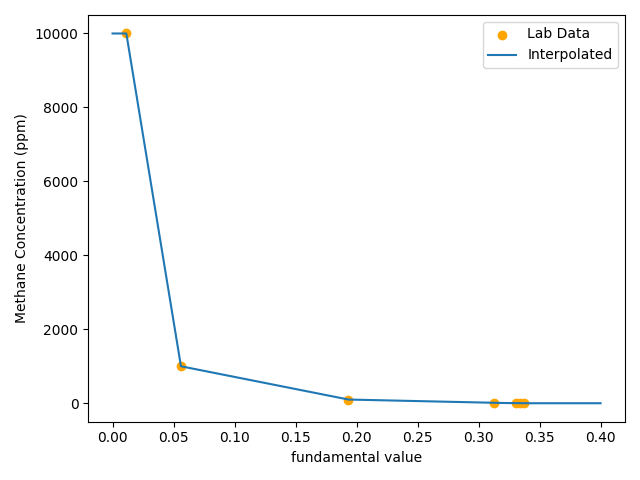
\includegraphics[width=0.6\textwidth]{figures/nopp_fundamental_calib_inverted.png}
    \caption{Fitted calibration curve for measurements of methane observed by Pythia.}
    \label{fig:nopp_curve}
\end{figure}

Compensation of Pythia's time response was also performed on post-calibrated data using the methodology described in \cite{miloshevich2004development} with a smoothing window of 5 minutes, and subsampling at a quarter of the time delay window. This methodology is sensitive to noise in the signal, which motivates the extreme sub-sampling that is performed. Fig.~\ref{fig:fund_corrected} shows the effect of smoothing, time-correction, and conversion on the direct signal recorded by Pythia before normalization. 

\begin{figure}[h!]
    \centering
    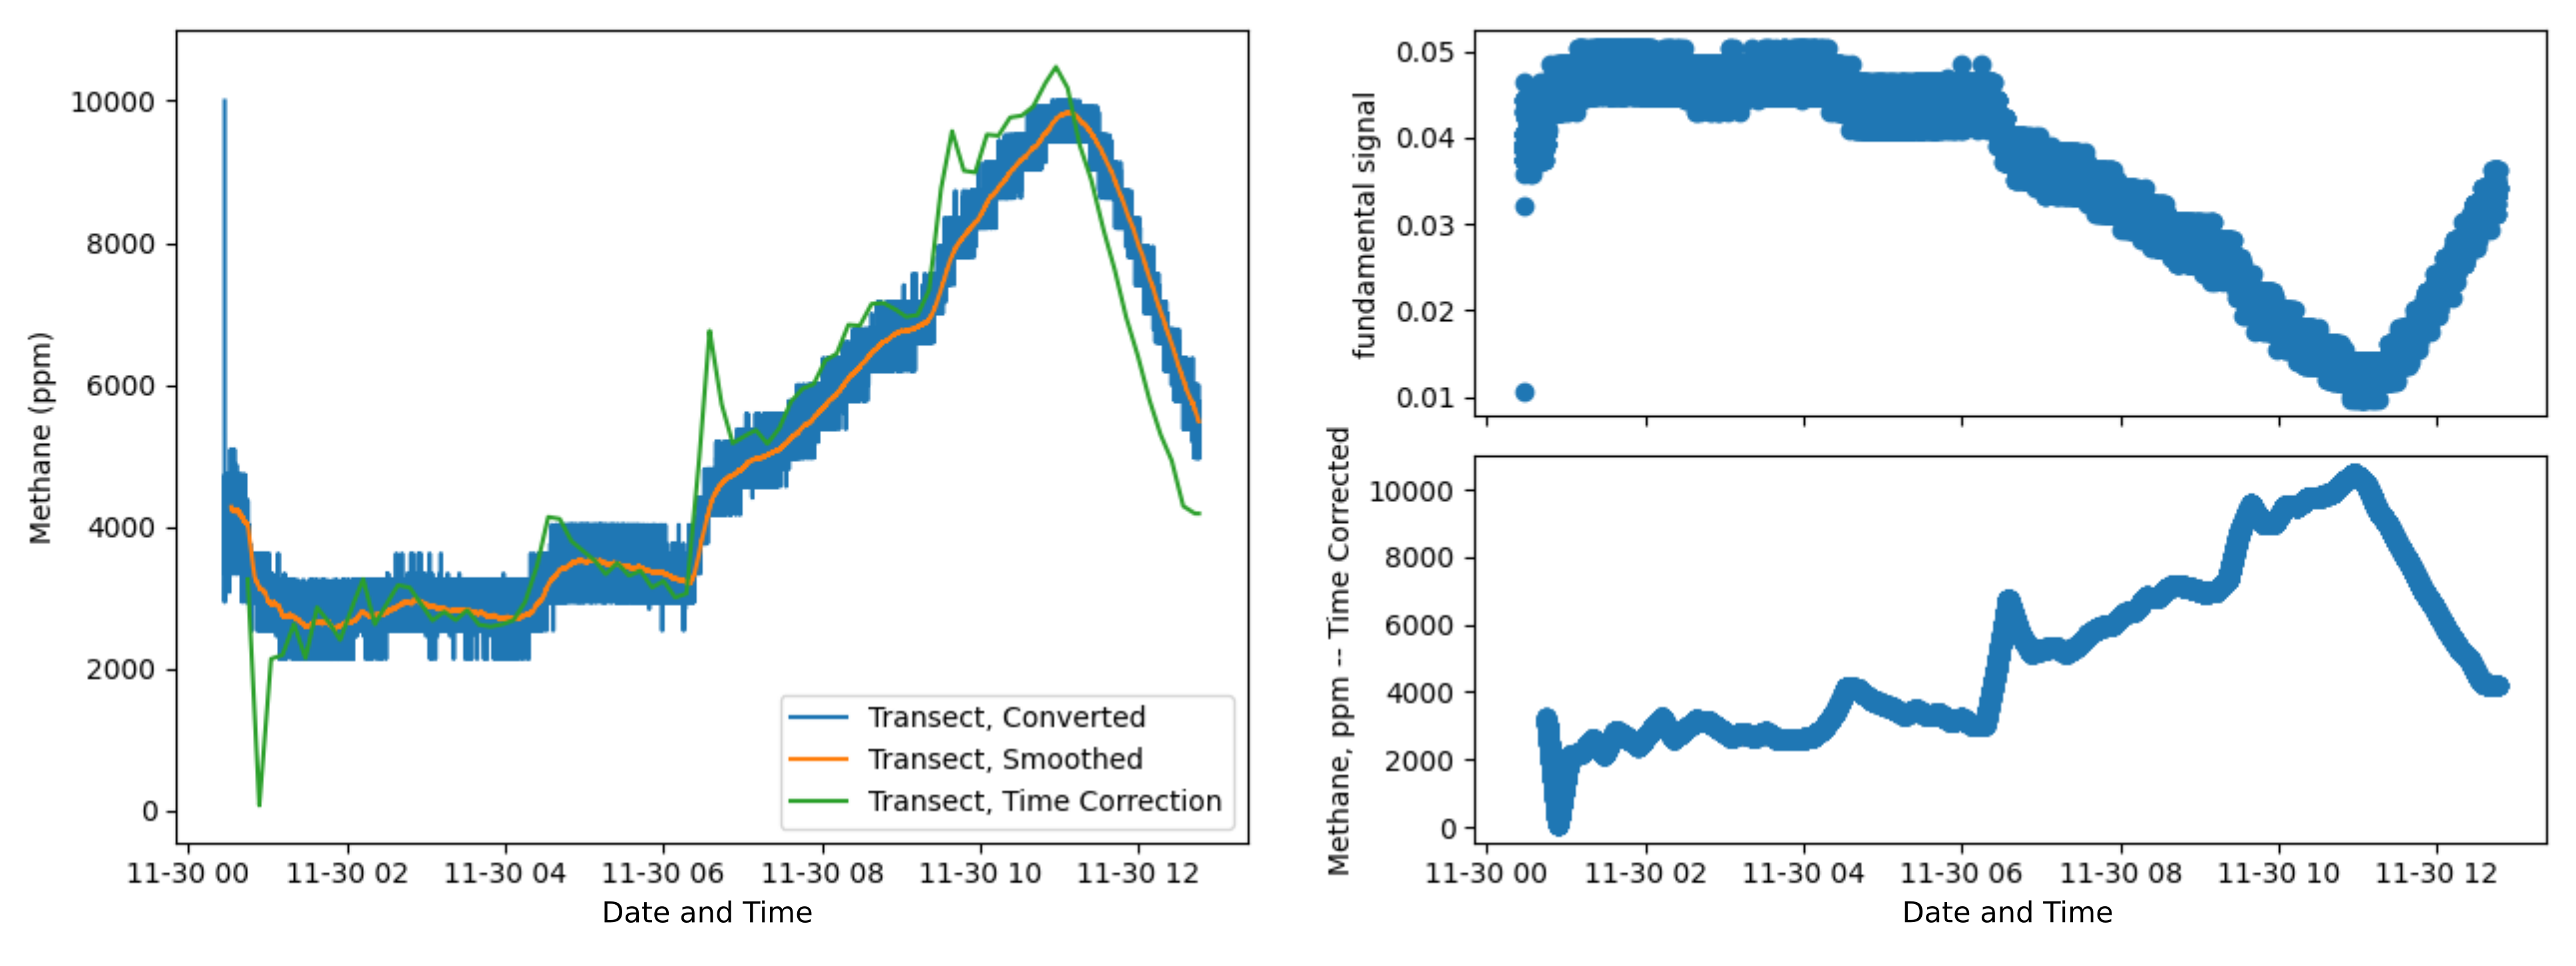
\includegraphics[width=1\textwidth]{figures/pythia_calibration.png}
    \caption{Calibration curve, smoothing, and time correction applied to Pythia observations during the transect, before reported normalization in the manuscript.}
    \label{fig:fund_corrected}
\end{figure}


\section{Depth-Correction}
\label{app:perception:depth}
Temperature, salinity, and oxygen are expected to be weakly stratified in the deep ocean. To remove these effects from data collected by AUV Sentry and the rosette, we fit a line to the average observations collected within binned 20 m intervals of observed depth for each platform separately. Separately computing the correction for each instrument additionally controls for small discrepancies in calibration between the platforms. Fig.~\ref{fig:linear_fits} compares these lines with the observations collected.

\begin{figure}[h!]
    \centering
    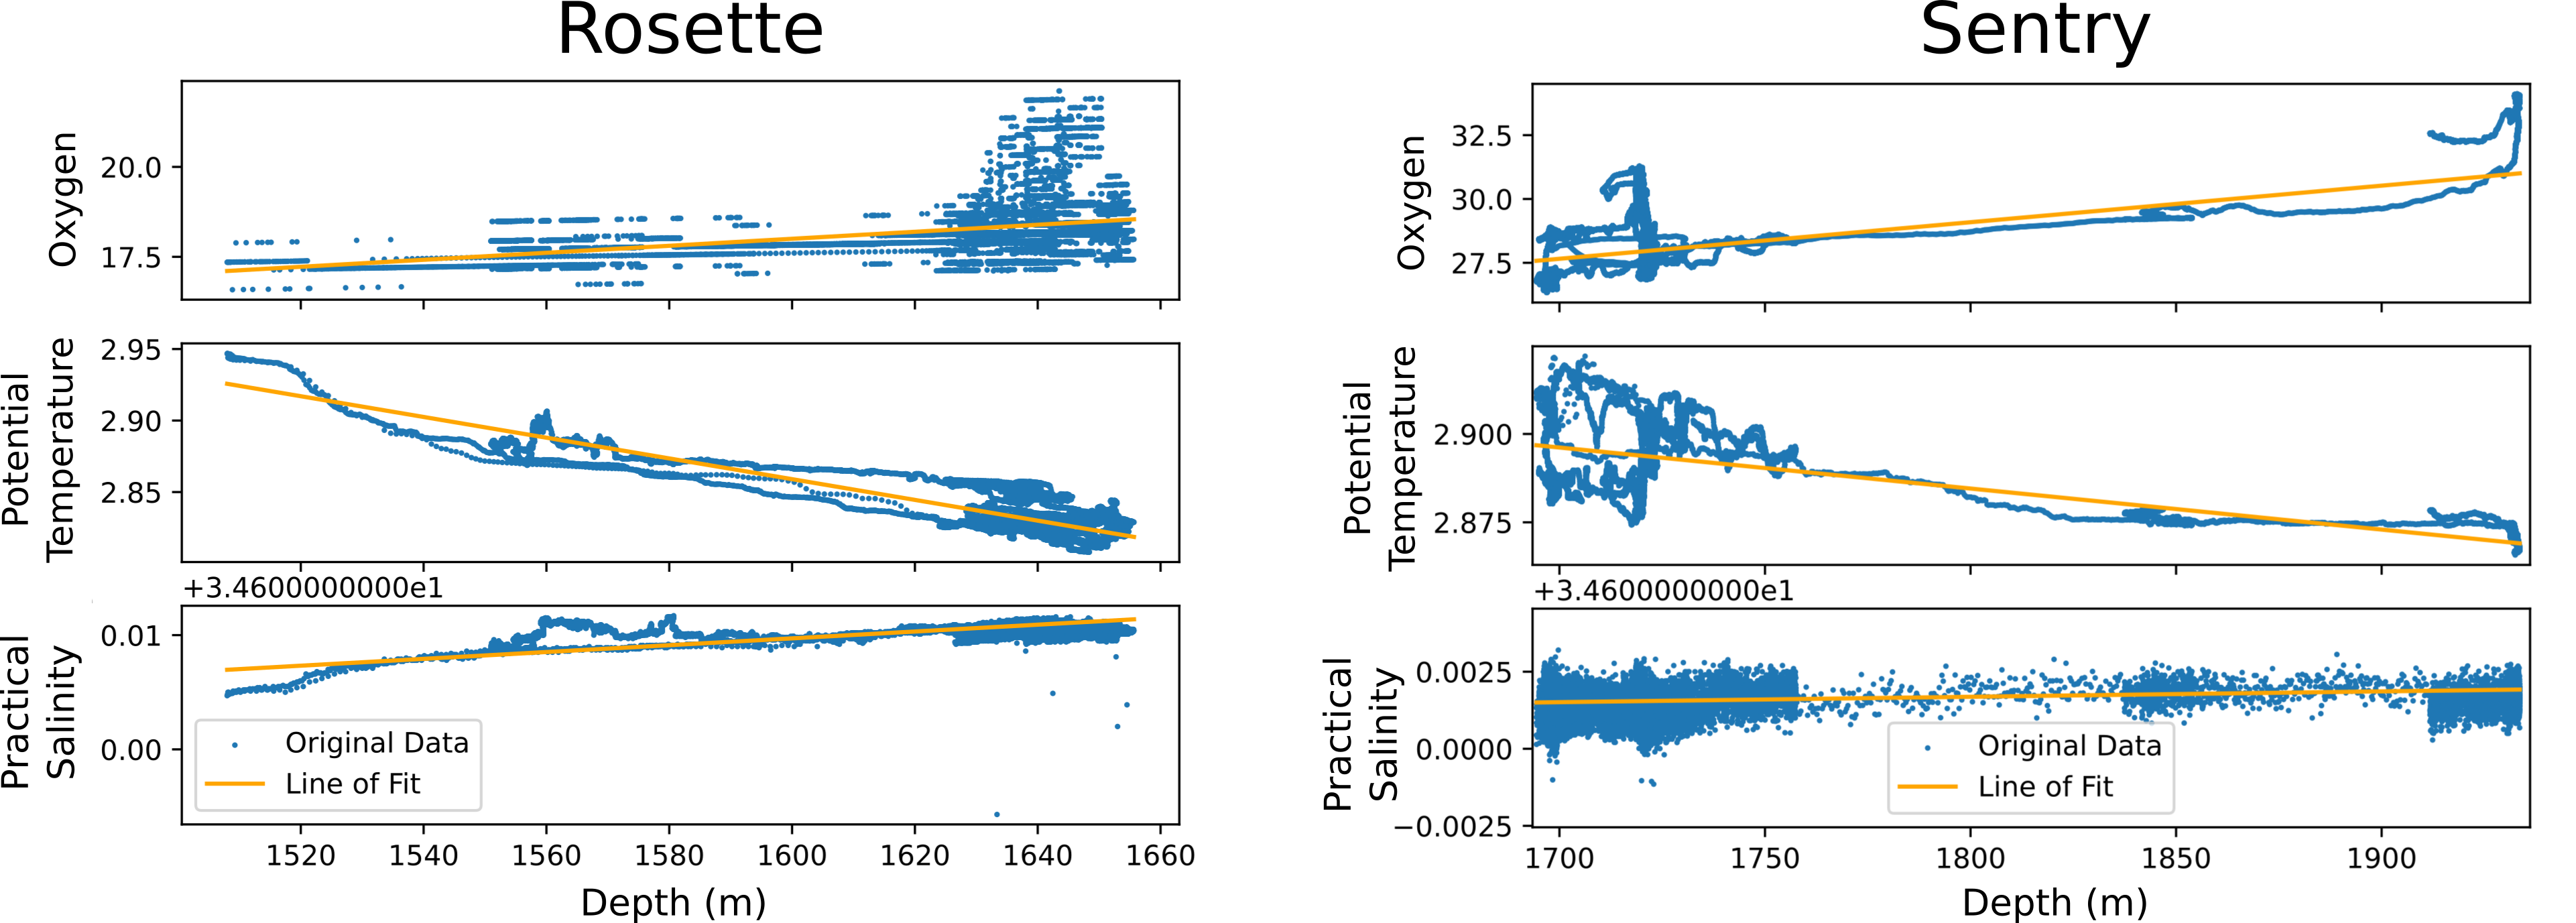
\includegraphics[width=1\columnwidth]{figures/depth_correction_plots.png}
    \caption{Linear functions are fit to data collected for oxygen, temperature, and salinity instruments on each platform separately. A residual value is then computed for each observation.}
    \label{fig:linear_fits}
\end{figure}

\section{Description of Plume Model for Transect Design}
\label{app:perception:model}
We adapted an idealized buoyant bent-plume model proposed by \cite{tohidi2016highly} for atmospheric bent plumes in a weakly stratified fluid in order to inform at what heights to deploy AUV Sentry and the rosette during the transect. We rewrite the system of equations provided in \cite{tohidi2016highly} as follows:

\begin{align}
    E &= \alpha\left|\frac{M}{Q} - u\cos(\theta)\right| + \beta\left|u\sin(\theta)\right| \\
    \frac{dQ}{ds} &= QE\sqrt{\frac{2(1 + \lambda^2)}{M\lambda}} \\
    \frac{dM}{ds} &= u\cos(\theta)\frac{dQ}{ds} + \frac{FQ}{M}\sin(\theta)\\
    \frac{d\theta}{ds} &= \left(\frac{FQ}{M}\cos(\theta) - u\sin(\theta)\frac{dQ}{ds}\right)\frac{1}{M}
\end{align}
\begin{align}
    \frac{dF}{ds} &= -QN^2\sin(\theta)\\
    \frac{dX}{ds} &= \cos(\theta)\\
    \frac{dZ}{ds} &= \sin(\theta)
\end{align}

\noindent where $E$ is a mixing entrainment coefficient which considers both vertical and horizontal mixing and is weighted by parameters $\alpha$ and $\beta$, $u$ is the crossflow velocity which can be a function of depth and time, $\lambda$ is a parameter which modifies the ellipse which describes the plume envelope, $Q$ is specific volume flux, $M$ is specific momentum flux, $F$ is specific buoyancy flux, $\theta$ is plume centerline trajectory angle, $s$ is the plume centerline trajectory, $X$ is distance along a coordinate axis aligned with the plume centerline, $Z$ is height with respect to plume source along a vertical axis, and $N^2$ is the Brunt-V\"ais\"al\"a frequency, computed with respect to the density gradient at the reference depths of the source and plume height.

The system of equations essentially yields a ``snapshot'' of a plume envelope at some moment in time. For time-varying crossflows, multiple snapshots can be computed for different moments in time (different crossflow orientations and magnitudes) and chained together in a common coordinate reference system in order to track a plume trajectory. For the purposes of determining which heights to deploy AUV Sentry and the rosette for the transect, we compute a prototypical envelope and use the estimated bent nonbuoyant plume height to set the transect depths/altitudes.

The initial conditions for solving this system of ordinary differential equations are set via estimates of vent characteristics including exit velocity, temperature, salinity, and area. Specifically:

\begin{align}
    Q_o &= \lambda V_v \frac{A_v}{\pi} \\
    M_o &= Q_o V_v \\
    F_o &= -g10^{-4}(T_v - T_z)Q_o \\
    \theta_o &= \frac{\pi}{2}
\end{align}

\noindent where $V_v$ is exit velocity at the vent orifice, $A_v$ is the vent orifice area, $T_v$ is the temperature at the orifice area, and $T_z$ is the expected temperature of ambient seawater at the estimated vent depth. Note that initial buoyancy flux is primarily driven by temperature changes, as we anticipate this to be the major driver of density gradients at our measurement scale. Expected salinity gradients could be similarly considered.

Estimated vent characteristics and crossflow were selected based on empirical observations of the deep sea vents located along the northern Guaymas Basin ridge and observations of current magnitude collected by a current tiltmeter deployed by ROV Jason during several days of the research cruise. Table~\ref{tab:params} lists the settings for planning the transect selected for these characteristics. Background salinity and temperature profiles were computed according to standard Pacific Ocean temperature and salinity functions as described in \cite{speer1989model}; additionally the equation of state for computing density profile from salinity and temperature measurements was used also as defined in \cite{speer1989model}. The prototypical plume is computed with a source located at 1850 m depth.

\begin{table}[h!]
    \centering
    \begin{tabular}{c|c|l}
        Parameter & Assignment & Description \\
        \hline
        $\lambda$ & 1.0 & Ratio of elliptical axes of the plume envelope \\
        $V_v$ & \SI{0.58}{\meter\per\second} & Exit velocity of fluids at vent orifice \\
        $A_v$ & \SI{0.82}{\meter\squared} & Area of vent orifice \\
        $T_v$ & \SI{340}{\celsius} & Temperature of fluids at vent orifice \\
        $\alpha$ & 0.15 & Longitudinal shear-driven mixing coefficient \\
        $\beta$ & 0.19 & Transverse shear-driven mixing coefficient \\
        $u$ & \SI{0.1}{\meter\per\second} & Magnitude of crossflow \\
    \end{tabular}
    \caption{Parameter, vent characteristics, and ambient crossflow setting used for transect design.}
    \label{tab:params}
\end{table}

The prototypical plume envelope computed in this manner estimates a nonbuoyant plume depth between 1570-1750 m (Fig.~\ref{fig:plume_envelopes}). AUV Sentry is altitude limited in order to keep a fix on the ocean floor for navigation; it is set to its maximum altitude of \SI{120}{\meter} in order to intersect with the bottom of the estimated nonbuoyant layer; this corresponds to a depth of approximately 1700 m throughout the basin. The rosette can be arbitrarily fixed to a height, but so as not to interfere with AUV Sentry operations and to sample a different point in the estimated nonbuoyant layer, a depth of 1650-1600 m was targeted.

\begin{figure}[h!]
    \centering
    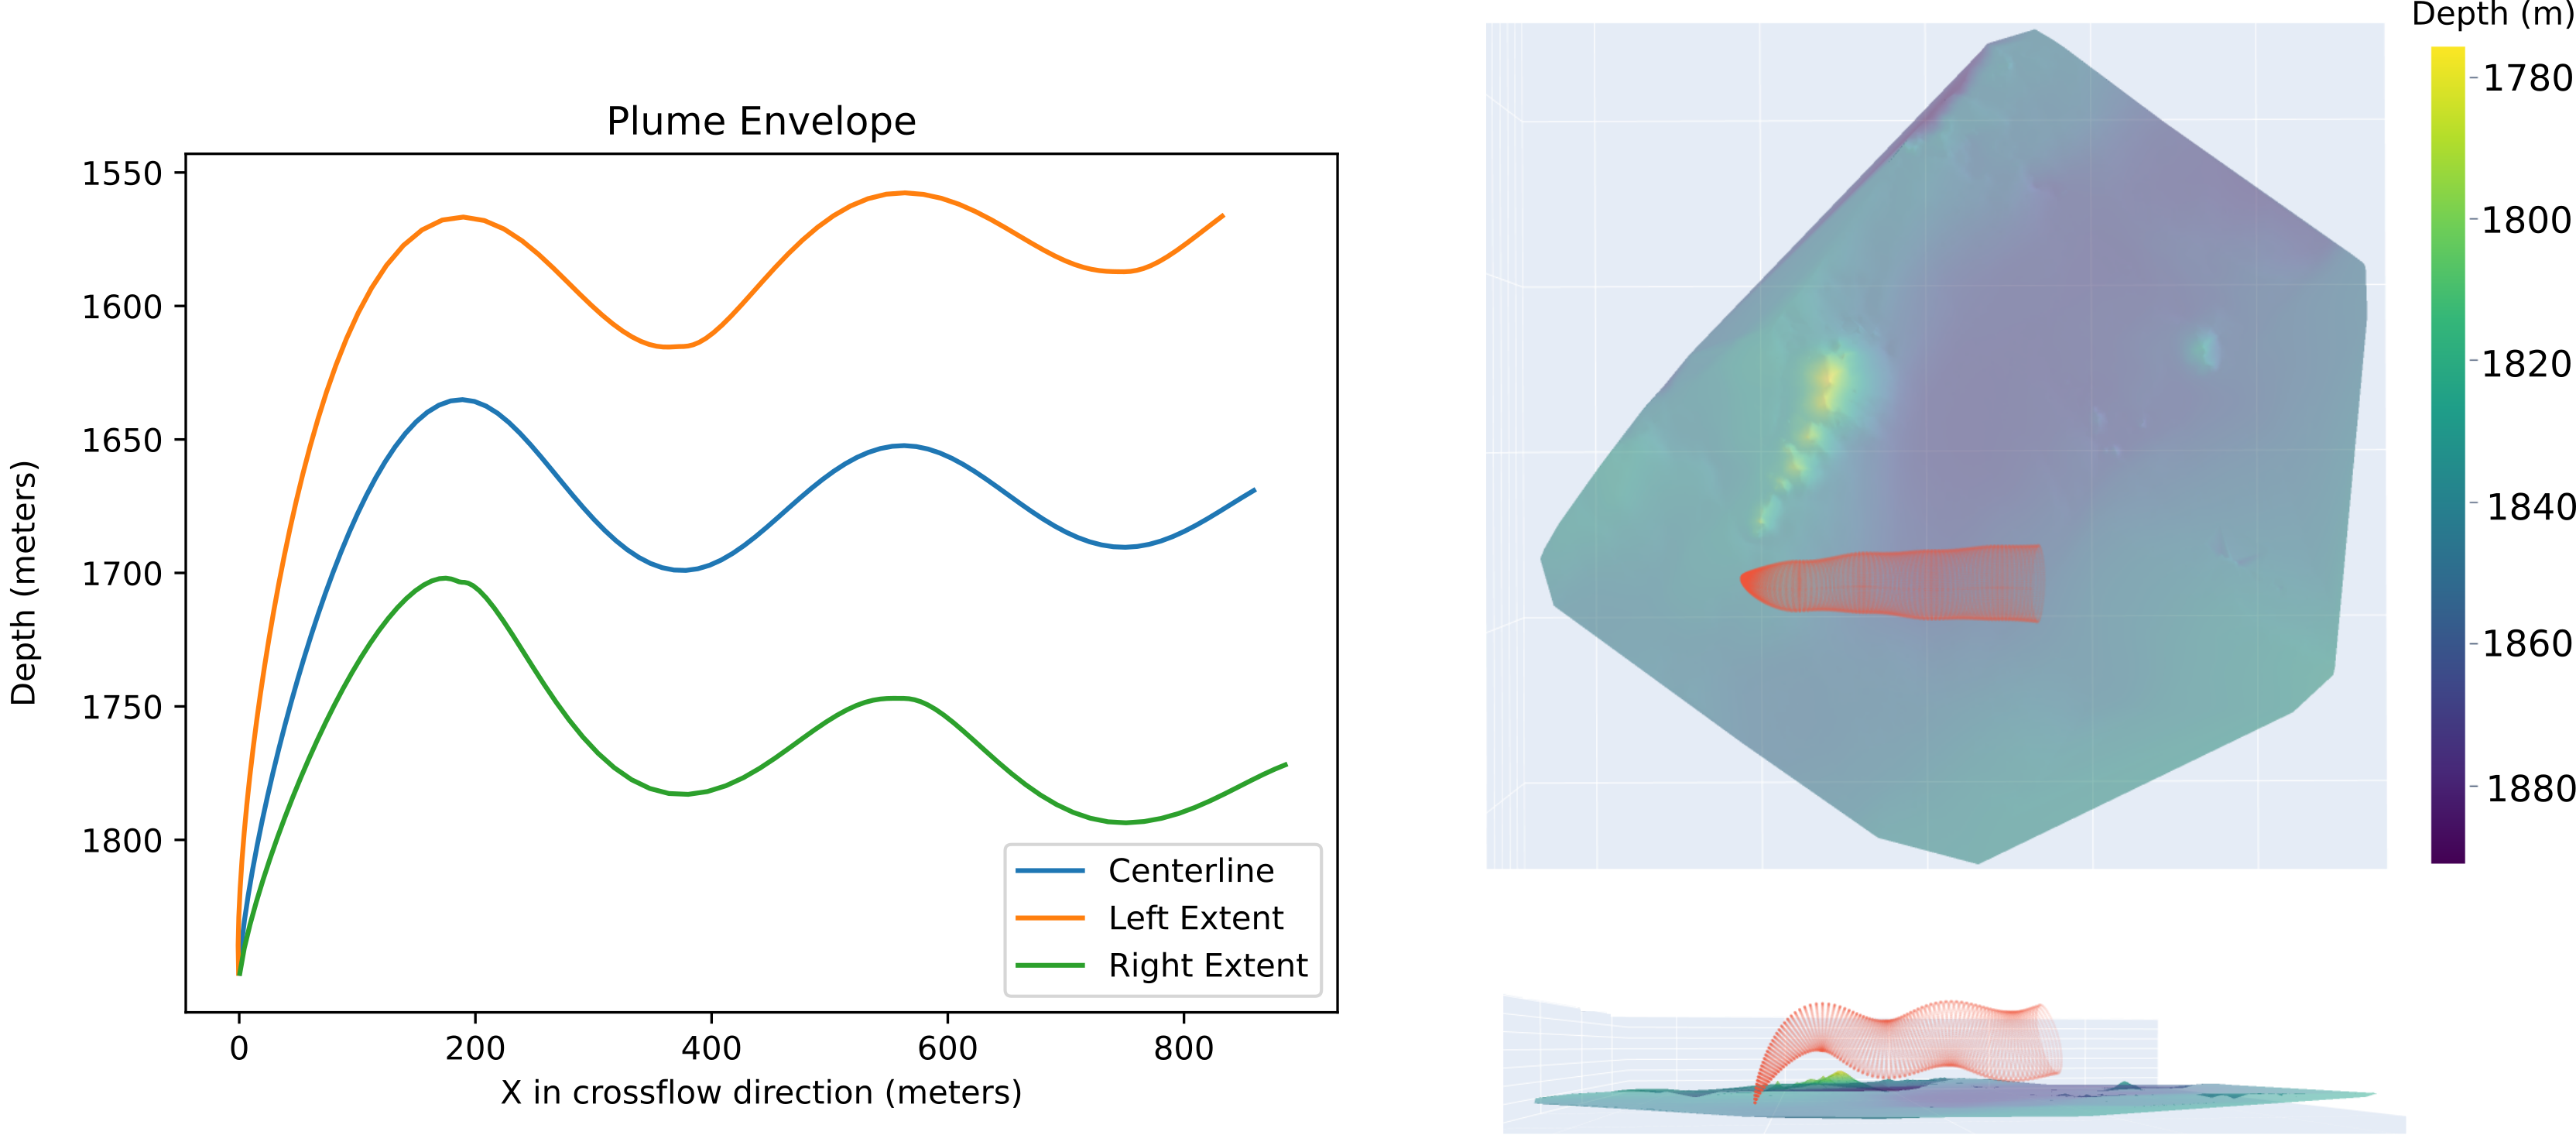
\includegraphics[width=1\columnwidth]{figures/plume_envelopes.png}
    \caption{A prototypical plume estimate according to the modified buoyant plume model in crossflow. The same envelope is plotted with respect to absolute depth (with a source located at 1850 m) on the left, and illustratively in the context of the hydrothermal ridge on the right.}
    \label{fig:plume_envelopes}
\end{figure}
